\documentclass[a4paper,11pt, titlepage, twoside]{article}
\usepackage[intoc, english]{nomencl}

%Cedit a tots els estudiants futurs
\title{Plantilla Per a TFG-TFM ETSEIB}
\author{Andrea Serrano Costafreda i Bartomeu Costa Prats }
\date{gener 2019}

\usepackage[utf8]{inputenc}

% Language and font encodings
\usepackage[english]{babel} %spanish, english, ...
\usepackage{lipsum}
\usepackage[utf8]{inputenc}
\usepackage[T1]{fontenc}
\usepackage{parskip}
\setlength{\parskip}{4mm}
\setlength{\footskip}{60pt}
\setlength{\headheight}{15pt}

%% Sets page size and margins MARGES IGUALS ALS DOS COSTATS
\usepackage[a4paper,top=3cm, bottom=3cm, inner=2cm, outer=2cm, footnotesep=1cm, heightrounded]{geometry}
% MARGES ORIGINALS
%\usepackage[a4paper,top=3cm, bottom=3.2cm, inner=3cm, outer=2cm, footnotesep=1cm, heightrounded]{geometry}

%% Useful packages

\usepackage{float}
\usepackage{verbatim}
\usepackage{amsmath}
\usepackage{systeme}
\usepackage{graphicx}
\usepackage{multirow}
\usepackage{caption}
\usepackage{subcaption}
\usepackage{wrapfig}
\usepackage[colorinlistoftodos]{todonotes}
\usepackage[colorlinks=true, allcolors=blue]{hyperref}
\usepackage{titlesec}
\usepackage{fancyhdr}
\usepackage[firstpage]{draftwatermark}
\usepackage{transparent}
\usepackage{textcomp} %podem escriure ``o'' amb la comanda \textdegree també € amb \texteuro
\usepackage[gen]{eurosym} %tb official en lloc de ``gen''
\usepackage[section]{placeins} %Evita que les figures saltin de secció
\usepackage{fancyref}
\usepackage{array}
\usepackage{longtable}
\usepackage{mathtools}
\usepackage{commath}
\usepackage{scrextend}%Indentar un bloc sencer
\usepackage{tgpagella}
\usepackage{dtk-logos}
\usepackage{nomencl} % Per a la nomenclatura
\usepackage{hyperref} % Per als links
\usepackage{tikz}
\usepackage{pgfgantt}
\usepackage{setspace}
\usepackage{circuitikz}
\usepackage{algorithm}
\usepackage{algpseudocode}
\usepackage{enumitem}

%------------------------------------------
% tikz things
\usetikzlibrary{shapes.geometric, arrows}

%------------------------------------------
\renewcommand{\baselinestretch}{1.25} 
%%Comentaris
\begin{comment}
Aquí podem posar tots els comentaris que calgui sense anar posant %
REFERENCIAT
\label{marker}, \ref{marker} and \pageref{marker} \footnote{footnote text}

\begin{addmargin}[esq]{dta}
El text d'aquí incrementa els seus marges segons ``esq'' i ``dta''
\end{addmargin}
\end{comment}

%------------------------------------------

%%Comença pàgina nova per cada Secció SI hi ha alguna cosa escrita a la anterior

%\newcommand{\sectionbreak}{\cleardoublepage}
\newcommand{\sectionbreak}{\clearpage}

% Descomentem això si volem començar les subseccions a pàgines noves
%% \newcommand{\subsectionbreak}{\clearpage}


%------------------------------------------

%%Caps de pagina i peus (E/O (even/odd), L/C/R (left/center/right) y H/F (header/footer))
\fancyhf{}
\fancyhead[ER]{Bachelor's thesis}
\fancyhead[OL]{Offshore wind park optimization}
\fancyhf[ELH, ORH]{pp. \thepage}
%\fancyfoot[C]{}
\fancyfoot[EL, OR]{

\includegraphics[scale=0.2]{imatges/ETSEIB.png}}
\pagestyle{fancy}
\raggedbottom

\SetWatermarkText{\hspace{9mm}\transparent{0.15}
\includegraphics[scale=2.5]{imatges/ETSEIB.png}}
\SetWatermarkAngle{0}
\SetWatermarkLightness{1}

% Text al inici de la nomenclatura
\makenomenclature
\renewcommand{\nompreamble}{The next list describes several abbreviations and symbols that will be later
used within the body of the thesis.}

\begin{document}
\renewcommand{\refname}{Bibliography}
\begin{titlepage}
    {\centering
    {\Huge Bachelor's Thesis}\\
    \vspace{5mm}
    {\Large \textbf{Bachelor's degree in Industrial Technologies and Economic Analysis}}\\
    \vspace{20mm}
    \Huge \textbf{Offshore Wind Park Optimization}\\
    \vspace{10mm}
    %\Huge\textbf{MEMÒRIA}\\
    \vspace{3mm}
    \Large\text{June 2024}\\  %Si en lloc del dia de la darrera edició es vol una data fixa, elimineu \today i poseu la data
    }
    \vspace{20mm}
    \hspace{2mm}
    \begin{tabular}{l@{ } l}
        \vspace{5mm}
        \Large \textbf{Author:} & \Large{Carles Roca Reverter} \\
        \vspace{5mm}
        \Large\textbf{Supervisor:} & \Large{Josep Fanals i Batllori}\\
        \vspace{5mm}
        \Large\textbf{Tutor:} & \Large{Oriol Gomis Bellmunt}\\
        
         \Large\textbf{Call: } & \Large{Spring 2023-2024}\\
    \end{tabular}\par
    \vspace{10mm}
    {\centering
    
\includegraphics[scale=0.3]{imatges/ETSEIB.png}\\
    {\Large Escola Tècnica Superior \\ d'Enginyeria Industrial de Barcelona}\\
    \vspace{3mm}
    
\includegraphics[scale=0.4]{imatges/UPC_logo.PNG}
    \par
    }
    \end{titlepage}
%\maketitle

\clearpage
\thispagestyle{empty}
\null\newpage 
\pagenumbering{arabic}

\section*{Abstract}

Short and must include results.

\textbf{Keywords:} offshore wind power plant, power flow, renewable energy, HVAC, transmission system, optimization, mixed-integer programming, genetic algorithms.


\textbf{MSC codes:} 90C11, 90C15, 90C29, 90C30, 90C59


\section*{Resum}
 
Short and must include results.

\textbf{Paraules clau:} parc eòlic marí, flux de potència, energia renovable, HVAC, sistema de transmissió, optimització, programació enter mixta, algoritmes genètics.


\textbf{Codis MSC:} 90C11, 90C15, 90C29, 90C30, 90C59
\section*{Resumen}

Short and must include results.

\textbf{Palabras clave:} parque eólico marino, flujo de potencia, energía renovable, HVAC, sistema de transmisión, optimización, programación entera mixta, algoritmos genéticos.


\textbf{Códigos MSC:} 90C11, 90C15, 90C29, 90C30, 90C59
%\clearpage\null\newpage

\tableofcontents

%\section{Nomenclature}

\nomenclature{AC}{Alternating Current}
\nomenclature{DC}{Direct Current}
\nomenclature{HVAC}{High Voltage Alternating Curent}
\nomenclature{HVDC}{High Voltage Direct Current}
\nomenclature{MVRSM}{Mixed-Variable ReLU-based Surrogate Modelling}
\nomenclature{N-R}{Newton-Raphson Method}
\nomenclature{OPF}{Optimal Power Flow}
\nomenclature{OSS}{Offshore Substation}
\nomenclature{OWF}{Offshore Wind Farm}
\nomenclature{OWPP}{Offshore Wind Power Plant}
\nomenclature{PF}{Power Flow}
\nomenclature{SCR}{Short Circuit Ratio}
\nomenclature{XLPE}{Cross-Linked Polyethylene}

\printnomenclature
\listoffigures
\listoftables




\section{Preface}

Argurably, climate change is one of the most pressing challenges we are facing today as humanity.
That's why I wanted to develop a project revolving around sustainable solutions for the 
energy system of the future. As an engineering student I wanted to explore how renewable 
energy sources can by integrated into the grid and what challenges it poses, that's why I 
contacted Oriol Gomis to explore thesis topics within this field.\par

He introduced me diverse research areas and also eRoots, a spin-off from the UPC-CITCEA
that develops software solutions for modern grid modelling, analyis and optimization. Then Josep Fanals, my supervisor
and eRoots CEO, presented to my various topics that they would be potenitially interested to develop a thesis on. This is when 
he introduced me to the topic of design, sizing and optimization of the transmission system of offshore wind power plants. The research 
group CITCEA-UPC has been working in this area \cite{paperbase} and further developement on this field was the breeding ground for this proposal.
The topic inmediatly caught my attention and that is how I ended up as an intern at eRoots developing software solutions for the optimization of offshore wind power plants.


\begin{figure}[H] %Recorda fixar la posició de les figures si no
	\centering
	
\includegraphics[width=0.15\textwidth]{imatges/ETSEIB.png}
	\caption{Una imatge del logo de l'ETSEIB}
	\label{fig:ETSEIB} %Si es posen les etiquetes de forma ordenada, la vida es més fàcil...
\end{figure}

Per referir-se a la Fig.\ref{fig:ETSEIB}.
Per no repetir informació és millor referir-se a altres apartats \ref{Optimization}.\par
I recorda, sempre és important citar a la bibliografia \cite{paperbase}.\\
La bibliografia ha d'estar ordenada, en teniu un exemple a la pàgina \pageref{biblio}
%------------------------------------------
\section{Introduction}\label{Introduction}

\subsection{Motivation}

During the industrial engineering studies you get in touch with a wide range of topics that can be applied
to different fields. During the last years to get introduced to electrical engineering fundamentals and its 
applications. I discovered a deep interests for those topics and realized is a key tool for ensuring a future towards
energy systems that can inegrate renwable energy sources.\par

The main driving force behind choosing this topic is the need to develop a sustainable energy system that can
ensure a future for the next generations. The energy system is a key player in the fight against climate change. Moreover, the last
report on global sustainable development \cite{SustGoal7} highlights how \textit{Goal 7: Affordable and clean energy} is failing to meet its targets.
In fact, it actually notices a backward trend in the 2020-2023 period when it comes to this goal targets, which signals that it is an area where efforts
have to be put in. \par

This thesis is my modest and passionate contribution to provide sustainable solutions for our future.

\subsection{Scope}

This work will limit its study to the optimal design of HVAC transmission systems, without considering the cost comparision with
HVDC.  Moreover, it will limit its study to the steady-state of balanced three phase load systems, without considering unbalanced or transient states.
\subsection{Objectives}

The main objectives of the thesis are the following:
\begin{itemize}
    \item Model all the elements of the transmission system of an offshore wind power plant and find its equivalent circuit.
    \item Implement a power flow solver with Python.
    \item Formulate the optimization problem to minimize all types of costs taking into account the technical constraints of the system. 
    \item Bencharmark different optimization algorithms thar find solutions faster than state of the art methods.
    \item Study some specific cases applicable to real offshore wind power plants.
  \end{itemize}

\newpage

\subsection{Outline}

The thesis is structured as follows:
\begin{itemize}
    \item Chapter \ref{Grid} introduces offshore wind power plants, the problem we want to tackle and models the elements that we find in a HVAC transmission system.
    \item Chapter \ref{Minimization}  formulates the minimization problem, including objective functions and constraints. In this section we also
    build the power flow solver that deals with the equality contraints and the algorithm for computing objective function values.
    \item Chapter \ref{Optimization} explains state of the art methods to solve the problem, its limitations, and our new approaches, involving
    genetic algorithms and  an optimal power flow approach.
    \item Chapter \ref{CaseStudies} showcases  the results for a specific case study and benchmarks the performance of the optimization algorithms.
    and computational time.
    \item Chapter \ref{Conclusions} collects the main outcomes of the thesis and proposes future lines of work.
    \item Chapter \ref{Planning} presents the planning and viability studies for the project.
\end{itemize}
%------------------------------------------
\section{Technical background: grid to study}\label{Grid}

\subsection{Offshore wind power plants}
As global energy demands surge and the pressing need for sustainable development becomes ever more urgent, 
the quest for renewable energy sources has intensified. Among these, wind power has emerged as a frontrunner due to its potential to generate substantial amounts of clean electricity.
While onshore wind farms have been widely implemented, their offshore counterparts are gaining increasing attention for their ability to harness the stronger and more consistent winds found over the oceans.\par

Offshore wind power, defined as the use of wind turbines located in bodies of water to generate electricity, presents several advantages over onshore installations. The primary benefit lies in the higher wind speeds
and lower turbulence experienced offshore, which contribute to greater energy yields. Additionally, offshore wind farms can be situated closer to urban centers located along coastlines, thereby reducing transmission
losses and enhancing energy efficiency. The development of offshore wind technology has seen rapid advancements in recent years. From the deployment of the first offshore wind farm in Denmark in 1991 to the establishment
of massive installations such as the Hornsea Project in the UK, the scale and capacity of these projects have grown significantly. Technological innovations, including larger turbines, floating foundations, and improved
grid integration techniques, have further propelled the industry forward.

\subsection{Transmission system: design and reactive power compensation problem}

When designing the transmission system of an OWPP, several factors must be considered to ensure optimal performance and efficiency. The system must be capable of transmitting the generated power from the wind turbines to the onshore grid
while trying to be as energy and cost-efficient as possible. There are two main types of technologies that can bu used, HVDC and HVAC. In this thesis we will focus our study to the HVAC technology.\par

To put in context the relevance of this topic, the work and software developed in this thesis will be used
as the breeding-ground of a parternship between eRoots and Acciona, a leading infrastructre company in Spain that has shown interest in developing a tool for the optimal design
of OWPP's transmission systems.

One drawback of using HVAC cables is the high shunt capcitance they have, which is even larger in underground cables,
which are the ones used for OWPP.

\begin{table}[h]
    \centering
    \begin{tabular}{|c|c|c|}
    \hline
     & Overhead Lines & Underground Lines \\
     \hline
    Capacitance per unit length ($\mu$F/km) & 0.01 - 0.02  & 0.3 - 0.6 \\
    \hline
    \end{tabular}
    \caption{Comparison of Capacitance per unit length of Overhead and Underground Lines}
    \label{tab:capacitance_comparison}
    \end{table}

The charging current of this capacitance limits the active power tranfer capacity of the line and increases
power losses and voltage across the line due to the Ferranti effect\cite{ferranti}. This effect can be described by the votage difference between the sending and reciving end of transmission line under no-load conditions:

\begin{equation}
    \frac{V_{o} - V_{i}}{V_{o}} = \omega^2CL\frac{l^2}{2}
\end{equation}
where $V_{o}$ and $V_{i}$ are the receiving and sending end voltages respectively, $\omega$ is the frequency, $C$ is the capacitance per unit length, $L$ is the inductance per unit length and $l$ is the length of the line. Note that the voltage difference is
proportional to the square of the length of the line which leads to overvoltages for long transmission lines.\par

However, the possbility to include reactive power compensation elements helps reduce the reactive power generation. Figure \ref{fig:whycomp} shows how including
this compensation reduces power losses, especially when we approach the no-load condition, which is equavialent to not having any type of active power injection from
the OWPP, i.e. the wind speed is very low.
\begin{figure}[h] %Recorda fixar la posició de les figures si no
	\centering
	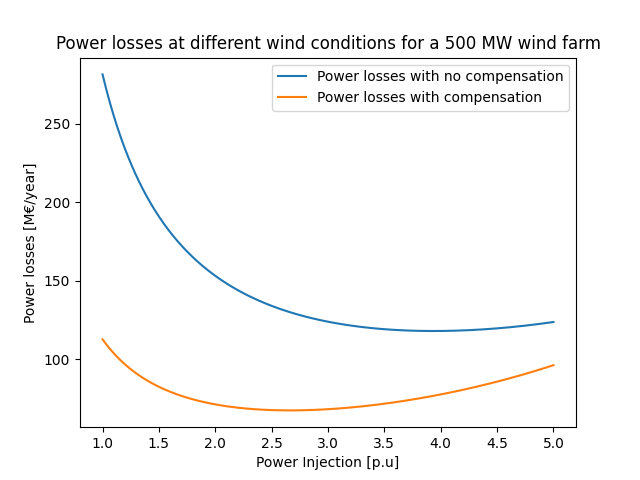
\includegraphics[width=0.65\textwidth]{imatges/why_compensation.png}
	\caption{Power losses comparision when including reactive power compensation}
	\label{fig:whycomp} %Si es posen les etiquetes de forma ordenada, la vida es més fàcil...
\end{figure}

The goal of the project is to determine where this compensation has to be placed  and how to size it. But this is only part of the design carachteristics we want to optimize. A full descrption of the optimitization variables will be
presented in Chapter \ref{Minimization}.

Taking all this into consderation, a HVAC transmission system layout for an OWPP with reactive power compensation looks like the one in Figure \ref{fig:fulltransmission}.
\begin{figure}[H] %Recorda fixar la posició de les figures si no
    \centering
    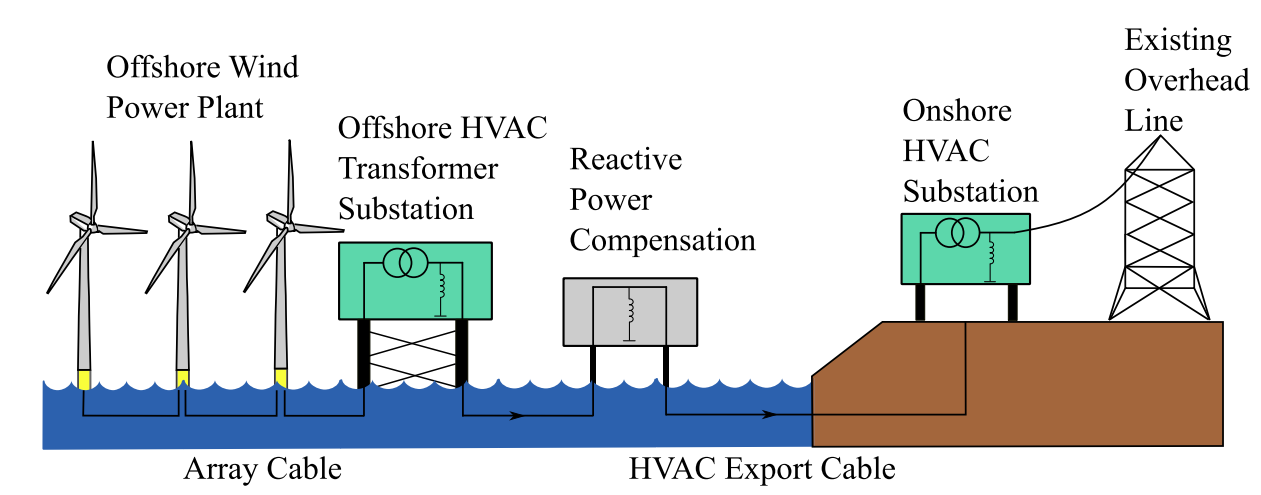
\includegraphics[width=0.75\textwidth]{imatges/layout.png}
    \caption{HVAC transmission system layout for an OWPP with reactive power compensation\cite{paperbase}}
    \label{fig:fulltransmission} %Si es posen les etiquetes de forma ordenada, la vida es més fàcil...
\end{figure}

From this general layout we will be able to create the network model using the equivalent circuits of the  elements involved.

\subsection{Grid elements}

To be able to do a steady-state analysis of the transmission system we need to model all the elements in the grid. This section models this elements and presents
some important concepts to understand the grid.




\subsubsection{Cables}

Cables are an essential part of HVAC transmission systems. We will consider  three-core cross-linked Polyethylene (XLPE) cables, which are the most common type of cables used in OWPP's. 



The equivalent circuit of a cable is shown in Figure \ref{fig:piline}. We will use a model

\begin{figure}[h]
\centering
\begin{circuitikz}
    \draw (0,0) to [generic, l=$\underline{Z}_{\pi}$] (6,0);
    \draw (1,0) to [generic, l=$\underline{Y}_{\pi}$] (1,-2);
    \draw (5,0) to [generic, l=$\underline{Y}_{\pi}$] (5,-2);
    \draw (0,-2) -- (6,-2);
\end{circuitikz}
\caption{Pi model transmission line}
\label{fig:piline} 
\end{figure}   

%\newpage
\subsubsection{Transformers}

\begin{figure}[h]
\centering
\begin{circuitikz}
    \draw (0,0) to [generic, l=$\underline{Z}_{tr}$] (6,0);
    \draw (1,0) to [generic, l=$\underline{Y}_{tr}$] (1,-2);
    \draw (0,-2) -- (6,-2);
\end{circuitikz}
\caption{Transformer model}
\label{fig:transformer}
\end{figure}

\subsubsection{Shunt reactor: reactive power compensation}
To compensate reactive power generation we will use shunt reactors. They are reactive power absorvers and in our case will be connected from
the line directly to the ground. The equivalent circuit is shown in Figure \ref{fig:shuntreactor}.
\begin{equation}
    \underline{y}_{sh} = \frac{1}{j\omega L}
\end{equation}
where $L$ is the inductance of the reactor.
\begin{figure}[h]
\centering
\begin{circuitikz}
    \draw (0,0) to [generic, l=$\underline{y}_{sh}$] (0,-3) node[ground]{};
    
\end{circuitikz}
\caption{Shunt reactor model}
\label{fig:shuntreactor}
\end{figure}

We will consider the possibility to include 5 different shunt reactors in the system. Further development on the reasoning of this scheme on \ref{fulltransmission}

\subsubsection{Main grid}
It will be the slack bus.

We will model the grid we are connected to using a Thévenin equivalent circuit where $\underline{u}_{g}$ is the
Thévenin voltage and $\underline{z}_{g}$ is the Thévenin impedance:
\begin{subequations}\label{maingrideq}
\begin{align}
    \underline{z}_{g} = R_g + jX_g \\
    R_g = \sqrt{\frac{\frac{U_{g}^2}{SCR} \, p_{owf}S_{base}}{(\frac{X_g}{R_g})^2+1}}
\end{align}
\end{subequations}
Note that we need the short circuit ratio ($SCR$) and the $\frac{X_g}{R_g}$ ratio as parameters to the equivalent circuit.
\begin{itemize}
    \item The $SCR$ is the ratio of the short circuit apparent power in the case of a line-line-line-ground
    fault at the location in the grid where some generator is connected to the power rating of the generator itself.
    It is somehow a measure of the grid strength to small disturbances.
\end{itemize}

\begin{figure}[h]
\centering
\begin{circuitikz}
    \draw (0,0) to[sV, l=$\underline{u}_{g}$] (0,-3) to (0,-3) node[ground]{};
    \draw (0,0) to [generic, l=$\underline{z}_{g}$](-2,0);   
\end{circuitikz}
\caption{Main grid model}
\label{fig:maingrid}
\end{figure}

\subsubsection{Power plant}
We will model our OWPP as a simple power injection at one end of the transmission line. For our
analysis we will consider that there is no reactive power generation, therefore $q_{owf} = 0$. $p_{owf}$ will be the active power generation that will depend 
on the wind conditions of the plant. The reach of the work will limit its analysis to a fix power generation.
\begin{figure}[h]
\centering
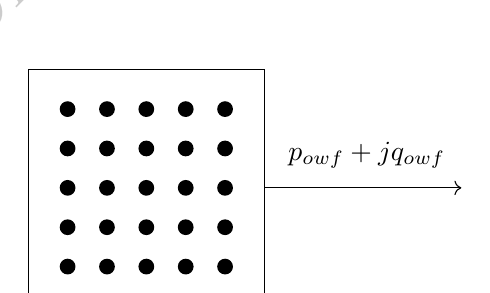
\begin{tikzpicture}
    \draw (0,0) rectangle (3,3);
    % Draw the dots
    \foreach \x in {0.5,1,1.5,2,2.5}
        \foreach \y in {0.5,1,1.5,2,2.5}
            \fill (\x,\y) circle (0.1);
    \draw[->] (3,1.5) -- (5.5,1.5);
    \node at (4.3,1.5)[label ={[font=\bfseries] above:$p_{owf}+jq_{owf}$}]{};
\end{tikzpicture}
\caption{Power plant}
\label{fig:powerplant}
\end{figure}
 Explicar aquí que differents vents, diferents potènices injectadees i referenciar a future work.
\newpage

\subsection{Costs modelling}
\subsubsection{Cables}

Equations from \cite{chalmers}:
\begin{align}
    C_{cables} &= n_{cables} (A + B \exp(\frac{CS_n}{10^8})) \cdot E_{\frac{eu}{sek}} \cdot \frac{1}{10^6} \quad \left[\frac{M\euro}{\text{km}}\right] \\
    S_n &= \sqrt{3}V_{rated}I_{rated} \quad \left[\text{VA}\right]
\end{align}



\subsubsection{Transformers}

\begin{equation}
    C_{tr}= 0.0427 \cdot S_{r-tr}^{0.7513} \quad \left[\frac{M\euro}{\text{km}}\right]
\end{equation}

\subsubsection{Shunt reactor}

\begin{equation}
    C_{sh}= K \cdot Q_l \cdot + P = K \cdot Y_l\cdot U_{AC-N}^2 + P \quad \left[\frac{M\euro}{\text{km}}\right]
\end{equation}

\subsubsection{Switchgears}

\begin{equation}
    C_{gis-AC} = 0.0117 \cdot U_{AC-N} + 0.0231 \quad \left[\frac{M\euro}{\text{km}}\right]
\end{equation}

\subsubsection{Substation platform}

\begin{equation}
    C_{ss-AC} = 2.534 + 0.0887 \cdot P_{owf} \quad \left[\frac{M\euro}{\text{km}}\right]
\end{equation}

\newpage

\section{Power flow analysis} \label{fulltransmission}

Now we can fully define the power flow analysis.  This approach will allow as to model the transmission system as a set of buses (or nodes)
interconnected by transmission links. This will allow as to solve for the steady-state powers and voltages of the system. This step is crucial to latter on
formulate our optimization since power flow equations will be the equality constraint of the optimization problem, \ref{eqconstr}, and the objective function will also depend on the solution of the power flow (PF).

\subsection{Types of buses}

In this section we will breifly describe what is a bus and what types we have.\par
Buses are points of the grid which either supplied by generators, \textit{generator buses}, or those without generators, \textit{load buses}. More formally, a $n$-bus system, $N=\{B_1,...,B_i,...,B_n\}$ where $N$ is the set of $n$-nodes, is defined as:

\begin{equation}
    \forall B_i \in N,
    \begin{cases}
        S_i = P_i + jQ_i, & \text{where } S_i \text{ is the apparent power at bus } i \\
        V_i = |V_i|e^{j\theta_i}, & \text{where } V_i \text{ is the complex voltage at bus } i
    \end{cases}
    %\forall i \in N,  \text{where } N={1,2,...,i,...,n}
\end{equation}

As we can see, for each bus $i$ we have 4 variables:

\begin{itemize}
    \item $P_i$ and $Q_i$ are the active and reactive power at bus $i$ respectively.
    \item $|V_i|$ and $\theta_i$ are the voltage magnitude and angle at bus $i$ respectively.
\end{itemize}

It is important to note that in general we cannot specify all the $P_i$'s independently since there is a constraint imposed by the need to balance active power. In our case, a transmission system with losses, which are unknown before the PF,
the sum of $P_i$'s must be equal to losses. To tackle this we will define one bus as the $slack$ bus, where power injection is left free. Taking all of this account, depeding on the variables are known and unknown for a cerain bus we can classify them as:
\begin{itemize}
    \item \textbf{Slack bus:} The slack bus is the reference bus of the system. It is the bus where the voltage magnitude and angle are known, typically $|V_i|= 1, \theta_i= 0 $.
    All other buses angles will be referenced to the $slack$. It is used to balance the active and reactive power in the system.
    \item \textbf{Generator bus (PV):} The generator bus is the bus where the active power and voltage are known
    \item \textbf{Load bus (PQ):} The load bus is the bus where the active and reactive power are known. The voltage magnitude and angle are unknown.
\end{itemize}
In summary:
\begin{table}[h]
    \centering
    \begin{tabular}{|c|c|c|c|}
        \hline
        & Slack Bus & PQ & PV \\
        \hline
        Voltage Magnitude ($|V_i|$) & Yes & No & Yes \\
        \hline
        Voltage Angle ($\theta_i$) & Yes & No & No \\
        \hline
        Active Power ($P_i$) & No & Yes & Yes \\
        \hline
        Reactive Power ($Q_i$) & No & Yes & No \\
        \hline
    \end{tabular}
    \caption{Known and unknown variables for each type of bus}
    \label{tab:bus_variables}
\end{table}





\subsection{Per unit system (p.u.)}

In power systems analysis, it is common to use the per unit system to normalize the magnitudes of the variables. This is very useful when we are dealing with several transformers and voltage levels. 
The per unit system is defined as:
\begin{equation}
    \text{Per unit value} = \frac{\text{Actual value}}{\text{Base value}}
\end{equation}

In our case we will use $S_{base} =100 \text{ MVA}$ and $V_{base} = \text{ transmission voltage in kV}$ as the base values. This means that the per unit system will be defined as:
\begin{equation}
    \begin{cases}
        I_{base} = S_{base}V_{base} \\
        Y_{base} = \frac{S_{base}}{V_{base}^2} \\
    \end{cases}
\end{equation}

Using the per unit system will be particularly useful for analyzing the results and for dealing with the inequality constraints \ref{inequality}.

\subsection{Grid model}

Now we have all the information neeeded to build our full model. In \cite{paperbase} they consider five possible postions for the shunt reactors, as seen in Figure \ref{fig:poss_position}. 
\begin{figure}[H]
    \centering
	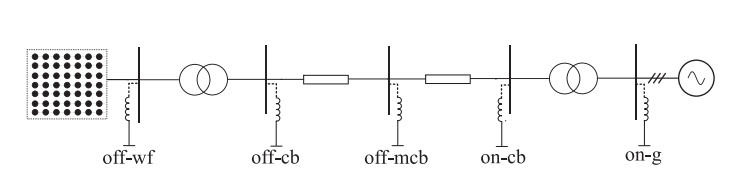
\includegraphics[width=0.65\textwidth]{imatges/poss_position.png}
	\caption{Possible locations for the shunt reactors \cite{paperbase}}
    \label{fig:poss_position}
\end{figure}



They consider when optimizing the cost function only the combinations where: if at a given transformer you place a reactor before it, you won't consider placing another one
after the same transformer. For sake of generality, we will consider that any combination within the five possible positions is valid. This will lead to a total of $2^5 = 32$ possible combinations.




\begin{figure}[h]
    \centering
    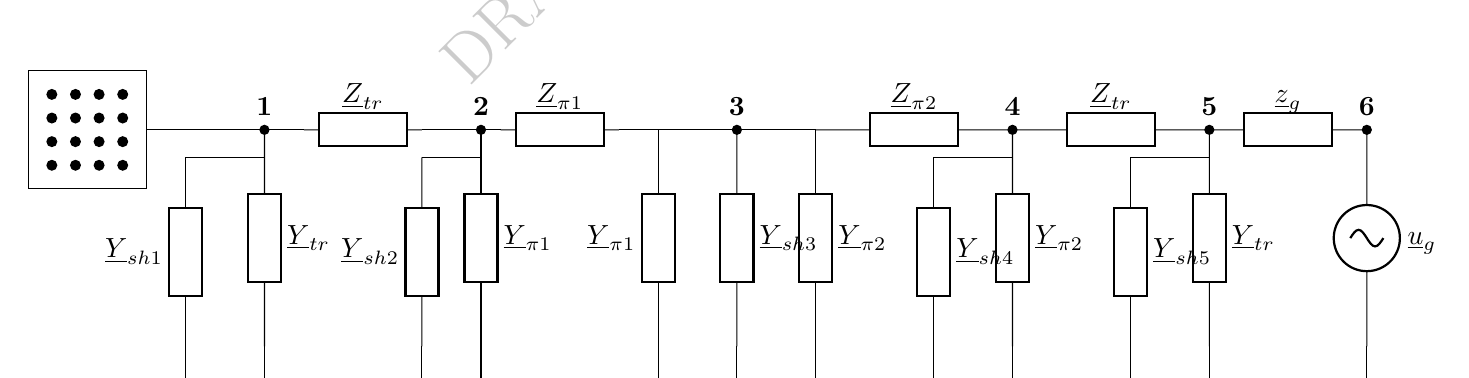
\begin{tikzpicture}[scale=1]
        \draw (0,0) rectangle (1.5,1.5);
        % Draw the dots
        \foreach \x in {0.3,0.6,0.9,1.2}
            \foreach \y in {0.3,0.6,0.9,1.2}
                \fill (\x,\y) circle (0.07);
        
        \draw (1.5,0.75) -- (3.5,0.75);
        \node at (3,0.75) [circle, draw=black, fill=black, inner sep=1pt, thick, label=above:$\textbf{1}$]{};
        \draw (3.5,0.75) to [generic, l=$\underline{Z}_{tr}$] (5,0.75);
        \draw (3,0.75) to [generic, l=$\underline{Y}_{tr}$] (3,-2) node[ground]{};
        \draw (3,0.4) -- (2,0.4);
        \draw (2,0.4) to [generic, l_=$\underline{Y}_{sh1}$] (2,-2)node[ground]{};
        \draw (5,0.75) -- (6,0.75);
        \node at (5.75,0.75) [circle, draw=black, fill=black, inner sep=1pt, thick, label=above:$\textbf{2}$]{};
        \draw (6,0.75) to [generic, l=$\underline{Z}_{\pi1}$] (7.5,0.75);
        \draw (5.75,0.75) to [generic, l=$\underline{Y}_{\pi1}$] (5.75,-2) node[ground]{};
        \draw (5.75,0.4) -- (5,0.4);
        \draw (5,0.4) to [generic, l_=$\underline{Y}_{sh2}$] (5,-2)node[ground]{};
        \draw (7.5,0.75) -- (10,0.75);
        \node at (9,0.75) [circle, draw=black, fill=black, inner sep=1pt, thick, label=above:$\textbf{3}$]{};
        \draw (8,0.75) to [generic, l_=$\underline{Y}_{\pi1}$] (8,-2) node[ground]{};
        \draw (9,0.75) to [generic, l^=$\underline{Y}_{sh3}$] (9,-2) node[ground]{};
        \draw (10,0.75) to [generic, l=$\underline{Y}_{\pi2}$] (10,-2)node[ground]{};
        \draw (10,0.75) to [generic, l=$\underline{Z}_{\pi2}$] (12.5,0.75);
        \draw (12.5,0.75) to [generic, l=$\underline{Y}_{\pi2}$] (12.5,-2) node[ground]{};
        \draw (12.5,0.4) -- (11.5,0.4);
        \node at (12.5,0.75) [circle, draw=black, fill=black, inner sep=1pt, thick, label=above:$\textbf{4}$]{};
        \draw (11.5,0.4) to [generic, l=$\underline{Y}_{sh4}$] (11.5,-2)node[ground]{};
        \draw (12.5,0.75) to [generic, l=$\underline{Z}_{tr}$] (15,0.75);
        \draw (15,0.75) to [generic, l=$\underline{Y}_{tr}$] (15,-2) node[ground]{};
        \node at (15,0.75) [circle, draw=black, fill=black, inner sep=1pt, thick, label=above:$\textbf{5}$]{};
        \draw (15,0.4) -- (14,0.4);
        \draw (14,0.4) to [generic, l=$\underline{Y}_{sh5}$] (14,-2) node[ground]{};
        \draw (15,0.75) to [generic, l=$\underline{z}_{g}$](17,0.75);
        \draw (17,0.75) to[sV, l=$\underline{u}_{g}$] (17,-2) to (17,-2) node[ground]{};
        \node at (17,0.75) [circle, draw=black, fill=black, inner sep=1pt, thick, label=above:$\textbf{6}$]{};
    

    \end{tikzpicture}
    \caption{Transmission system model and buses}
    \label{fig:fullgrid}
    \end{figure}

Now we choose where we want to define our buses and which type they are. We classify them as in Table \ref{table:bus_types}.
\begin{table}[h]
\centering
\begin{tabular}{c|c}
\hline
\textbf{Bus Number} & \textbf{Bus Type} \\
\hline
1 & PQ \\
2 & PQ \\
3 & PQ \\
4 & PQ \\
5 & PQ \\
6 & Slack \\
\hline
\end{tabular}
\caption{ Transmission system bus types}
\label{table:bus_types}
\end{table}

A brief explanation of the bus types is exposed:
\begin{itemize}
    \item \textbf{Bus 1:} It is the bus where the WPP is injecting power therefore active and reactive power are specified as $P_1=p_{owf}$ and $Q_1=q_{owf}$.
    \item \textbf{Bus 2, 3, 4, 5:} Those buses are plain  PQ load buses, where $P_i=0, Q_i=0$. We want to consider them as we will be interested in the voltage levels in the lines in order
    to compute possible over and undervoltages in the cables, as we will see in Chapter \ref{Minimization}.
    \item \textbf{Bus 6:} We will use this one as the slack bus. Note that this bus power flow solution for $P_6$ will allow us to compute the losses in the system
    and will be essential part of the optimization problem. Also, since we define it as the slack bus, it will be the reference for the voltage angles and in charge of balacinf the power in the transmission system. 
\end{itemize}
\subsection{Admittance matrix}

The admittance matrix encodes all the information of the elements of the grid and the relationship between them and allows us to perform the steady-state 
analysis of the grid.
Now we can build the full HVAC trasnsmission system model and fins its admittance matrix $\underline{Y}_{bus}$, which will be essential
for the power flow solver.

Using the Kirchhoff's Current Law (KCL):
\begin{equation}
\textbf{I} = \textbf{Y}_{bus} \textbf{V}
\label{eq:kirchhoff}
\end{equation}

where $\textbf{I}$ is the vector of injected currents, $\textbf{Y}_{bus}$ is the admittance matrix and $\textbf{V}$ is the vector of bus voltages.

Since we will be using the per unit system:
\begin{equation}
    y_i = \frac{Y_i}{Y_{base}}
\end{equation}

Note that when will build it, we take the series impedances in \ref{fig:fullgrid}, compute their inverse and add the subindex $s$ to identify them. For example:
\begin{equation}
    \underline{y}_{\pi1s} = \frac{1}{\underline{z}_{\pi1}}
\end{equation}

%We build $\underline{Y}_{bus}$ by inspection 

    
\begin{equation} \label{ybus}
    \resizebox{0.92\textwidth}{!}{%
    $\mathbf{{Y}_{bus}}=\begin{bmatrix}
        (\underline{y}_{tr}+\underline{y}_{trs}+\underline{y}_{sh1}) & -\underline{y}_{trs} & 0 & 0 & 0 & 0\\
       -\underline{y}_{trs} & (\underline{y}_{\pi1}+\underline{y}_{\pi1s}+\underline{y}_{sh2}+\underline{y}_{trs}) & -\underline{y}_{\pi1s} & 0 & 0 & 0  \\
       0 & -\underline{y}_{\pi1s} & (2\underline{y}_{\pi1}+2\underline{y}_{\pi1s}+\underline{y}_{sh3}) & -\underline{y}_{\pi2s}   & 0 & 0 \\
       0 & 0 & -\underline{y}_{\pi2s} & (\underline{y}_{\pi2}+\underline{y}_{\pi2s}+\underline{y}_{sh4}+\underline{y}_{trs}) & -\underline{y}_{trs} & 0  \\
       0 & 0 & 0 & -\underline{y}_{trs} & (\underline{y}_{tr}+\underline{y}_{tr}+\underline{y}_{sh5}+\underline{y}_{g}) & -\underline{y}_{g}  \\
       0 & 0 & 0 & 0 & -\underline{y}_{g} & \underline{y}_{g}\\
       \end{bmatrix}$
    }
\end{equation}

Some properties of the admittance matrix are:
\begin{itemize}[itemsep=0pt]
    \item It is a square matrix of size $n \times n$, where $n$ is the number of buses in the system.
    \item It is symmetric.
    \item The diagonal elements, $Y_{ii}$, are self-admittance, equal to the sum of the admittances of elements connected to bus $i$.
    \item $Y_{ij}$ is the negative of the admittance between buses $i$ and $j$
    \item  For our system, the sparcity is $\frac{20}{36}= 56\%$. Nevertheless, for large networks, the matrix es very sparse. The level of sparsity, which is the percentage of zero elements in a matrix, increases with the size of the network.
    For instance, in a 1000-bus system, the matrix approximately is 99\% sparse You can take advantage (and it will be essential to do it for very big networks!) of this sparsity using computational techniques \cite{sparcity}.
\end{itemize}

\subsection{Grid parameters}

We will use the following set of grid elements parameters for the transformers and the main grid:
\begin{table}[h]
    \centering
    \renewcommand{\arraystretch}{1.2}
    \begin{tabular}{l|c}
    \hline
    \textbf{Parameter} & \textbf{Value} \\
    \hline
    $SCR$ & \ 5 \\
    $\frac{X_g}{R_g}$ & 10 \\
    $P_{Cu}^{loss}$ & 60 kW \\
    $P_{Fe}^{loss}$ & 40 kW \\
    $u_k$ & 18 \%  \\
    $i_o$ & 1.2 \% \\
    \hline
    \end{tabular}
    \caption{Grid parameters \cite{paperbase}}
    \label{tab:gridparameters}
    \end{table}


\subsection{Power flow }
\subsubsection{Power flow equations}

We first going to derive an expression for the PF equations.
From \ref{eq:kirchhoff} we can get the injected current for the $i$-th component:
\begin{equation}
    I_i = \sum_{j=1}^{n} Y_{ik}V_k \quad i = 1,2,...,n
\end{equation}
Now we can compute the $i$-th bus power:
\begin{equation}
    S_i = V_iI_i^* = V_i\sum_{k=1}^{n} Y_{ik}^*V_k^* \quad i = 1,2,...,n
\end{equation}

Now if fe let $V_i = |V_i|e^{j\theta_i}$, and $Y_{ik} = G_{ik} + jB_{ik}$, we can write the power at bus $i$ as:
\begin{equation}
    S_i = \sum_{k=1}^n|V_i||V_k|e^{j\theta_i}(G_{ik} - jB_{ik}) = \sum_{k=1}^n|V_i||V_k|(cos(\theta_{ik})+jsin(\theta_{ik}))(G_{ik} - jB_{ik}) \quad i = 1,2,...,n
\end{equation}

Note that the real part of the admittance, $G_{ik}$, is the conductance and the imaginary part, $B_{ik}$, is the susceptance. Now if we separate the real and imaginary parts of the power we get:

\begin{align}
    P_i= \sum_{k=1}^n|V_i||V_k|(G_{ik}cos(\theta_{ik}) + B_{ik}sin(\theta_{ik}))\label{powerflowP} \quad i= 1,2,...,n \\
    Q_i= \sum_{k=1}^n|V_i||V_k|(G_{ik}sin(\theta_{ik}) - B_{ik}cos(\theta_{ik}))\label{powerflowQ} \quad i= 1,2,...,n
\end{align}  


\subsubsection{Newton-Raphson Solver}

\paragraph{Problem Solvability}

First, we have to make sure that our set of equations is solvable. First, if we strip away the $slack$-bus, we have 5 $PQ$-buses remaing. Each $PQ$-bus introduces 2 unknows, $|V_i|$ and $\theta_i$, and 2 equations, $P_i$ and $Q_i$. This means that we have 10 equations and 10 unknowns. 
After solving the system, from \ref{powerflowP} and \ref{powerflowQ} we can solve for the power injections of the slack bus, $P_6$ and $Q_6$. Hence, the condition for solvability is fullfiled.

To solve a set of non-linear equations, numerical methods are the standalone way to go. For the PF, on of the most used methods is the Newton-Raphson (N-R) method \cite{NRusual}. A brief description of this method will be presented for the $n$-dimentional case, but further descreiption can be found in \cite{llibrebase}.

We will descibe the process considering an $n$-bus system with all PQ buses except one slack bus. Note that in our specific case this conditions are met and $n = 6$. Once we strip away the slack bus, it remains to finnd the unknowns in the right side of equations \ref{powerflowP} and \ref{powerflowQ}. Therefore it will be convinient to
define the following vectors of unknowns of PQ-buses:
\begin{equation}
\begin{aligned}
    \mathbf{\theta} &= \begin{bmatrix}
    \theta_1 \\
    \theta_2 \\
    \vdots \\
    \theta_{n-1}
    \end{bmatrix} &
    \mathbf{|V|} &= \begin{bmatrix}
    |V_1| \\
    |V_2| \\
    \vdots \\
    |V_{n-1}|
    \end{bmatrix} &
    \mathbf{x} &= \begin{bmatrix}
    \mathbf{\theta} \\
    \mathbf{|V|} \\
    \end{bmatrix}
\end{aligned}
\end{equation}

Now the dependency between the power flow equations and the vector of unknowns $\mathbf{x}$ can be easily shown:
\begin{subequations}
\begin{align}
    P_i = P_i(\mathbf{x}) \quad i = 1,2,...,n-1 \\
    Q_i = Q_i(\mathbf{x}) \quad i = 1,2,...,n-1
\end{align}       
\end{subequations}

The N-R method is an iterative method that starts with an initial guess of the unknowns, $\mathbf{x}_0$, and then iterates the vector $\mathbf{x}$ until the right side matches the left side of the equations. Therefore we
can define the power mismatch vector $\mathbf{f(x)}$ as:
\begin{equation}
\begin{aligned}
    \mathbf{f(x)} = \begin{bmatrix}
    P_1(\mathbf{x}) - P_1 \\
    \vdots \\
    P_{n-1}(\mathbf{x}) - P_{n-1} \\
    Q_1(\mathbf{x}) - Q_1 \\
    \vdots \\
    Q_{n-1}(\mathbf{x}) - Q_{n-1}
    \end{bmatrix} = \begin{bmatrix}
    \mathbf{\Delta P(\mathbf{x})} \\
    \mathbf{\Delta Q(\mathbf{x})}
    \end{bmatrix} = \mathbf{0}
\end{aligned}
\end{equation}


Now we have to consider $\mathbf{J}$, the Jacobian matrix of $\mathbf{f(x)}$. For clarity, is convininet to parition $\mathbf{J}$ as:
\begin{equation}
\begin{aligned}
    \mathbf{J} = \begin{bmatrix}
    \mathbf{J_{11}} & \mathbf{J_{12}} \\
    \mathbf{J_{21}} & \mathbf{J_{22}}
    \end{bmatrix} = \begin{bmatrix}
        \frac{\partial \mathbf{\Delta P}}{\partial \mathbf{\theta}} & \frac{\partial \mathbf{\Delta P}}{\partial \mathbf{|V|}} \\
        \frac{\partial \mathbf{\Delta Q}}{\partial \mathbf{\theta}} & \frac{\partial \mathbf{\Delta Q}}{\partial \mathbf{|V|}}
    \end{bmatrix} = \begin{bmatrix}
    \frac{\partial \mathbf{P}}{\partial \mathbf{\theta}} & \frac{\partial \mathbf{P}}{\partial \mathbf{|V|}} \\
    \frac{\partial \mathbf{Q}}{\partial \mathbf{\theta}} & \frac{\partial \mathbf{Q}}{\partial \mathbf{|V|}}
    \end{bmatrix}
\end{aligned}
\end{equation}

if interest check derivation of the partial derivatives of the power flow equations with respect to the unknowns check the \hyperref[Appendix]{Appendix}.

Now it just remain to find the step $\Delta \mathbf{x^v}$ to update $\mathbf{x}$ solving the following linear system by Gauss elimination:
\begin{equation}
    \mathbf{J^k}\Delta \mathbf{x^k} = -\mathbf{f(x^k)}
\end{equation}

Now we update $\mathbf{x^{k+1}}=\mathbf{x^{k}}+\Delta \mathbf{x^k}$ and iterate until it converges. The convergence criteria is usually set as the maximum of the absolute value of the power mismatch vector, $\max(\mathbf{f(x)})$, is less than a tolerance, $tol$.







The N-R solver has been implemented in Python(check the \hyperref[Appendix]{Appendix}) and the procedure can be found in Algorithm 1.
\begin{algorithm}[H]
    \caption{Newton-Raphson Method}
    %\begin{algorithmic}[1]
    \begin{algorithmic}
    \Procedure{run\_pf}{}
        \State Initialize $V$ with ones and $\theta$ with zeros
        \Statex \hspace{\algorithmicindent}Set $V[slack$] to $1$, $\theta[slack]$ to $0$
        \Statex \hspace{\algorithmicindent}Set $P_{}$, $Q_{}$ based on OWPP data
        \Statex \hspace{\algorithmicindent}Set $iter = 0 $, $tol$ and $k = 0$
        \While{$iter$ < $max\_iter$ and $ \Delta PQ > tol$}
            \State Compute $P\_present$, $Q\_present$ using $V$, $\theta$, $Y_{bus}$
            \State Compute mismatch $\Delta PQ = [dP, dQ]$ as difference between calculated and given $P$, $Q$
            \State Compute the Jacobian matrix $J$.
            \State Solve the linear system $J \cdot \Delta x_k = -\Delta PQ$.
            \State Compute the updated $x^{k+1} = x^{k} + \Delta x^k $.
            \State Update $V$, $\theta$ using $dP$, $dQ$, $Y\_bus$
            \If{$\max(\Delta PQ) < tol$}
                %\State Converged
                \State \textbf{break}
            \EndIf
            
        \EndWhile
        \State \textbf{return} $V$, $\theta$
        \State Compute $P_{slack}$, $Q_{slack}$
    \EndProcedure
    \end{algorithmic}
    \end{algorithm}

Finally note that close to the solution vector $\mathbf{x^{*}}$ it can be proven that N-R normally presents
quadratic convergence \cite{convergenceNR}.


\section{Optimization problem formulation}\label{Minimization}

Explicar pq separem en multiobjective, ventages respsecvte solució tradicional, etc
\begin{equation}\label{vecunk}
    \resizebox{0.9\textwidth}{!}{%
    $\mathbf{x} = 
    \begin{bmatrix}
    vol_{tr}, & n_{cables}, & react_{bi_1}, &, ... &, react_{bi5}&, react_{cont1}&, ... &,react_{cont5}&, react_{bi5}&, S_{trafo}  
    \end{bmatrix}$
    }
\end{equation}

In equation \ref{vecunk} we define the vector of unknowns that we want to find the optimal values for. The vector includes the voltage of the transformer, the number of cables ...

\subsection{Objective function: multiobjective and mixed-integer}


\subsection{Constraints}
\subsubsection{Equality: Power Flow}

Now we define de equality constraints as seen in  Eq. \ref{eqconstr}
\begin{gather}
    \mathbf{h_m(x) = 0 } \label{eqconstr} \\
    \mathbf{S_i} = \mathbf{V_i(\sum_{j=1}^{N_{nodes}}Y_{ij}V_j)^*} \\
    \underline{s}_1-(p_{owf}+jq_{owf}) = 0, \nonumber \\
    \underline{s}_1-\underline{u}_1[(2\underline{y}_{tr}+\underline{y}_l)\underline{u}_1-(\underline{y}_{tr})\underline{u}_2]^* = 0, \nonumber \\
    \underline{s}_2-\underline{u}_2[-(\underline{y}_{tr})\underline{u}_1+(2\underline{y}_{\pi1}+\underline{y}_l+\underline{y}_{tr})\underline{u}_2-(\underline{y}_{\pi1})\underline{u}_3]^* = 0, \nonumber \\
    \underline{s}_3-\underline{u}_3[-(\underline{y}_{\pi1})\underline{u}_2+(2\underline{y}_{\pi1}+2\underline{y}_{\pi2}+\underline{y}_{l})\underline{u}_3-(\underline{y}_{\pi2})\underline{u}_4]^* = 0, \nonumber \\
    \underline{s}_4-\underline{u}_4[-(\underline{y}_{\pi2})\underline{u}_3+(2\underline{y}_{\pi2}+\underline{y}_l+\underline{y}_{tr})\underline{u}_4-(\underline{y}_{tr})\underline{u}_5]^* = 0, \nonumber \\
    \underline{s}_5-\underline{u}_5[-(\underline{y}_{tr})\underline{u}_4+(2\underline{y}_{tr}+\underline{y}_l+\underline{y}_{g})\underline{u}_5]^* = 0
\end{gather}

\newpage



\subsubsection{Inequality: Technical constraints}\label{inequality}

\begin{gather}
    \mathbf{g_n(x)\leq0} \\
    U_{kj}-U_{max}\leq0 \\
    U_{min}-U_{kj}\leq0 \\
    I_{kj}-I_{max}\leq0 \\
    Q_{min}-Q_{gj}\leq0 \\
    Q_{gj}-Q_{max}\leq0 \\
    Y_{l-ij}-Y_{l-i}^{max}\leq0 \\
    N_{react}-N_{react}^{max}\leq0 \\
\end{gather}

\newpage
\subsection{Algorithm overview}
H




\section{Optimization methods}\label{Optimization}

\subsection{State of the art: interior point method}
\subsection{NSGA-II: Genetic algorithm}
\subsection{Optimal Power Flow approach for compensation sizing}
h
\section{Results: Case study}\label{CaseStudies}

\subsection{500 MW OWPP}
%\subsubsection{50km}
%\subsubsection{100km}
%\subsubsection{150km}
%\subsection{1000 MW OWPP}
%\subsubsection{50km}
%\subsubsection{100km}
%\subsubsection{150km}
h

%------------------------------------------
\section{Conclusions}\label{Conclusions}
\subsection{Outcome}
\subsection{Future work}
h
%------------------------------------------
\section{Planning and viability studies}\label{Planning}

\subsection{Time Planning}

Figure \ref{fig:gantt} shows the time distribution for the tasks carried out in the thesis.
\begin{figure}[h]
\begin{center}
\begin{ganttchart}[hgrid, vgrid]{1}{20}
    \gantttitle{Thesis Gantt Chart}{20} \\
    \gantttitle{February}{4} \gantttitle{March}{4} \gantttitle{April}{4} \gantttitle{May}{4} \gantttitle{June}{4} \\
    \ganttbar{Literature review}{1}{6} \\
    %\ganttlinkedbar{Task 2}{2}{3} \ganttnewline
    \ganttbar{Modelling of the grid}{3}{7} \\
    \ganttbar{Power flow solver}{6}{8} \\
    \ganttlinkedbar{Optimization methods}{9}{18} \\
    %\ganttbar{Optimization methods}{9}{18} \\
    \ganttbar{Case studies}{12}{18} \\
    \ganttbar{Thesis final writting}{17}{20}
\end{ganttchart}
\caption{Thesis Gantt Chart}
\label{fig:gantt}
\end{center}
\end{figure}

\subsection{Economic assessment}

\begin{table}[h]
\centering
\begin{tabular}{l|c}
\hline
\textbf{Concept} & \textbf{Cost} \\
\hline
Computer & \$XXX \\
Working hours & \$XXX \\
Tutor supervision & \$XXX \\
\hline
\textbf{Total without IVA} & \$600 \\
\hline
\textbf{Total with IVA (21\%)} & \$720 \\
\hline
\end{tabular}
\caption{Thesis Costs}
\label{tab:costs}
\end{table}

\subsection{Environmental assessment}

This environmental assessment evaluates the energy costs incurred during
the development of a thesis over five months, using a computer as the primary tool. The primary energy consumption arises
from the computer's usage, which includes writing, research, data analysis, and communication.\par

Assuming an average laptop with a power consumption of 60 watts, used for approximately 6 hours daily, the total energy consumption
over five months is around 54 kWh. This consumption translates to roughly 30 kg of CO2 emissions, assuming the average emission
factor for electricity generation.\par

To reduce these energy costs and associated environmental impacts in future thesis projects, several strategies can be employed.
Utilizing energy-efficient computers, enabling power-saving modes, and limiting usage time can significantly lower consumption.
Additionally, adopting renewable energy sources, such as solar panels for charging devices, further reduces the carbon footprint,
contributing to a more sustainable academic practice.

\subsection{Social and gender equality assessment}

This assessment evaluates the social and gender equality aspects of a bachelor's thesis focused on developing a tool for optimizing renewable energy system design, authored by a 22-year-old white engineering student. While the thesis itself addresses a critical area in sustainable development, examining its social dimensions is essential to ensure inclusivity and equality.

The demographic profile of the author reflects broader trends in STEM fields, where women and minority groups remain underrepresented. This lack of diversity can influence the perspectives and priorities embedded in the research. Ensuring diverse representation in such projects is crucial for incorporating a wide range of insights and addressing the needs of various communities.

To promote social and gender equality, the research should consider the differential impacts of renewable energy systems on diverse populations. Inclusive design processes involve consulting with and incorporating feedback from women, marginalized communities, and other underrepresented groups. This approach ensures that the developed tools and technologies are accessible and beneficial to all segments of society.

Moreover, educational institutions should encourage and support participation from diverse backgrounds in engineering and renewable energy fields. Mentorship programs, scholarships, and targeted recruitment can help bridge the gender and social gap, fostering an environment where innovative solutions for renewable energy are developed through diverse and inclusive contributions.
%------------------------------------------


\section*{Acknowledgements}
 \addcontentsline{toc}{section}{Acknowledgements}

Primer de tot vull agraïr profundament el suport constant del Josep, el meu tutor, que m'ha donat consell i ajuda quan
l'he necessitada cada dia des de que vaig entrar a eRoots. Per extensió, agraïr la rebuda i suport de tot l'equip d'eRoots durant aquests mesos,
especialment a l'Oriol Gomis que ha proporcionat noves idees i enfocs al desenvolupament de la tesi.\par

Aquest TFG tanca un capítol de quatre anys de la meva vida que han sigut molt feliços gràcies als meus amics del grau; gràcies a tots nou. 
Finalment, agraïr a la meva família i a la Mire el seu suport incondicional cada dia i a ensenyar-me a estimar.
 %INICI BIBLIOGRAFIA
 
 \begin{thebibliography}{99}\label{biblio}
 \addcontentsline{toc}{section}{Bibliography}
 

 \bibitem{SustGoal7}
 \textit{Global Sustainable Development Report (GSDR) 2023}, United nations, 2023. [Online]. 
 Available: \href{https://sdgs.un.org/gsdr/gsdr2023}{Global Sustainable Development Report (GSDR) 2023}
 
 \bibitem{paperbase} 
 {J. Dakic, M. Cheah-Mane, O. Gomis-Bellmunt, and E. Prieto-Araujo},
\textit{“HVAC Transmission System for Offshore Wind Power Plants Including
 Mid-cable Reactive Power Compensation: Optimal Design and Comparison to VSC-HVDC transmission"}, \textit{IEEE Trans. Power Del.}, vol. 36,
 no. 5, pp. 2814–2824, Oct. 2021.
 %\texttt{Consultat \emph{quotiens necesse est}} 
 \bibitem{ferranti} 
 {W. Wiechowski and P. B. Eriksen},
\textit{“Selected studies on offshore wind farm
cable connections - challenges and experience of the Danish TSO"}, \textit{Proc.
IEEE Power Energy Soc. General Meet.: Convers. Del. Elect. Energy the
21st Century}, PES, 2008, pp. 1–8.

\bibitem{llibrebase} 
 {Arthur R. Bergen, Vijay Vittal},
\textit{“Power systems analysis"}, 2nd ed. Tom Robbins, 2000.

\bibitem{sparcity}
{Kenneth Nazimek},
\textit{“Sparcity and decoupling in load flow analysis"}, New Jersey Insitute of Technology, 1977.

\bibitem{NRusual}
{ Raquel García-Blanco}
\textit{"Efficient solvers for power flow equations: parametric solutions with accuracy control assessment"}, Doctoral thesis, UPC, 2016.


\bibitem{convergenceNR}
{Goran Andersson},
\textit{"Modelling and Analysis of Electric Power Systems"}, ETH - Power Systems Laboratory, 2008.

\bibitem{chalmers}
{Stefan Lundberg},
\textit{"Performance comparision of wind park configurations"}, Chalmers University of Technology, 2003.




\end{thebibliography}
 
\section*{Appendix}\label{Appendix}
\addcontentsline{toc}{section}{Appendix}

In the following link you can find the Git repository with all the code used for the development of this work:
\url{https://github.com/Ch4rlieStone/tfg_eroots}
 
\end{document}
